\section{The Sangria HM Dataset}
\label{sec:dataset}

We test our search methods on the LISA Data Challenge dataset~\cite{Baghi:2022ucj, LDC_WEBSITE}.
The LISA Data Challenges are designed to provide comprehensively modelled data as an introduction
to LISA data analysis. The dataset considered here is Challenge 2a, also known as
\textit{Sangria-HM}~\cite{LDC_WEBSITE_SANGRIA_HM}.
This dataset is similar to Challenge 2: Sangria~\cite{LDC_WEBSITE_SANGRIA, le_jeune_2022_7132178};
it contains exactly the same sources but uses a different waveform model, \texttt{PhenomHM}~\cite{}
... \gscd{A couple more sentences of introduction to sangria}

In applying our pre-merger search to the Sangria dataset, our first consideration is to check whether
the data has similar noise properties to our assumptions in our previous work. 
Figure~\ref{fig:psds} shows the PSD  

\begin{figure*}
    \centering
    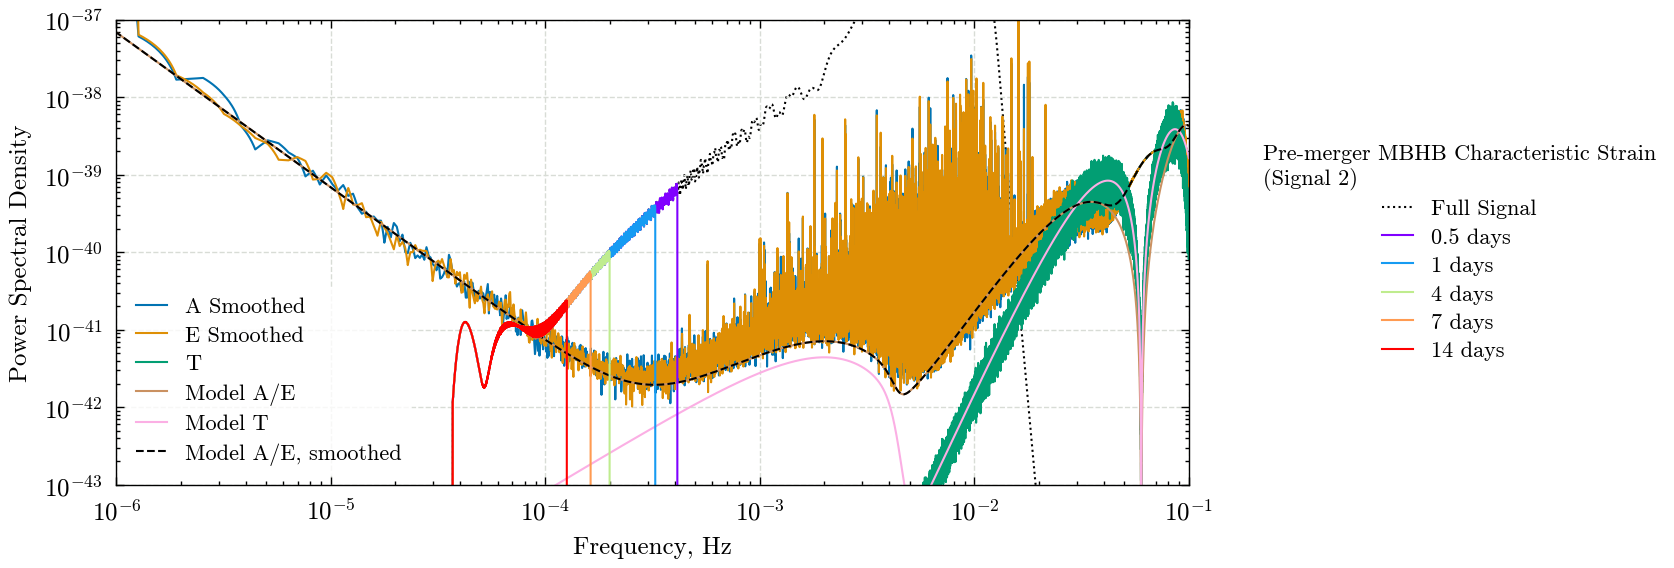
\includegraphics[width=\textwidth]{images/dataset/figure_X_psds_with_sources.png}
    \caption{
        Comparison of PSDs used in this work.
        The PSD is estimated from the Sangria dataset using the welch method with a segment duration of 18.25 days.
        The model shown is the noise model used to produce the Sangria dataset, and includes unresolvable galactic binary sources.
        Both the model and the estimated PSD require smoothing over the dip to zero at 0.06Hz.
        This smoothing is done using a Hann window to transition between the original PSD and a straight line between the peaks of the PSD model either side of the dip.
        We also show the characteristic strain for a representative MBHB signal from Sangria (Signal 2), which shows that at 14, 7 and 4 days-before-merger, the MBHB does not overlap
        the galactic binary confusion noise in frequency, but when the signal reaches around one day before merger,
        the galactic binary confusion noise starts to overlap with the signal.
    }
    \label{fig:psds}
\end{figure*}

\begin{table}
    \begin{tabular}{|cc|c|ccccc|}
\hline
\multicolumn{2}{|c|}{Signal}& \multicolumn{6}{c|}{Expected SNR} \\
\hline
Number & Time  & Full Signal & 0.5 & 1 & 4 & 7 & 14 \\
\hline
0 & 55.56 & 2699.04 & 70.99 & 52.74 & 24.33 & 16.43 & 9.51 \\
1 & 101.23 & 105.72 & 3.99 & 2.49 & 0.79 & 0.47 & 0.28 \\
2 & 129.26 & 400.25 & 10.76 & 7.51 & 2.91 & 1.84 & 1.07 \\
3 & 130.31 & 1992.38 & 71.92 & 54.76 & 27.52 & 19.88 & 13.22 \\
4 & 133.41 & 3475.28 & 115.99 & 88.26 & 44.02 & 31.65 & 20.46 \\
5 & 138.55 & 427.13 & 16.40 & 10.79 & 3.85 & 2.37 & 1.22 \\
6 & 157.61 & 673.48 & 24.99 & 16.19 & 5.48 & 3.25 & 1.55 \\
7 & 191.34 & 579.12 & 15.72 & 10.70 & 4.02 & 2.56 & 1.49 \\
8 & 199.60 & 365.18 & 16.21 & 10.68 & 3.77 & 2.28 & 1.11 \\
9 & 215.34 & 392.96 & 18.69 & 12.41 & 4.75 & 3.12 & 1.82 \\
10 & 236.41 & 2187.78 & 45.09 & 31.90 & 12.71 & 8.13 & 4.37 \\
11 & 257.27 & 1200.55 & 45.32 & 33.31 & 13.99 & 8.92 & 4.71 \\
12 & 271.29 & 359.02 & 21.27 & 14.71 & 6.10 & 4.17 & 2.57 \\
13 & 282.51 & 823.00 & 24.75 & 18.00 & 7.81 & 5.23 & 3.00 \\
14 & 341.62 & 230.57 & 9.88 & 6.43 & 2.22 & 1.34 & 0.67 \\
\hline
\end{tabular}

    \caption{
        Characteristic SNRs for signals in the Sangria dataset.
        These are computed by comparing characteristic strain for the signal to the
        noise model PSD.
        We see that Signal 1 is unlikely to be seen even 0.5 days pre-merger, and 
        that only the loudest signals - 0, 3, 4, 10, 11 and possibly 12, 13 - would be seen 4 days before merger.
    }
    \label{tab:characteristic_strain_snr}
\end{table}

\subsection{Smoothing the PSD}
PSD goes to zero at 60mHz - problem!

\begin{figure}
    \centering
    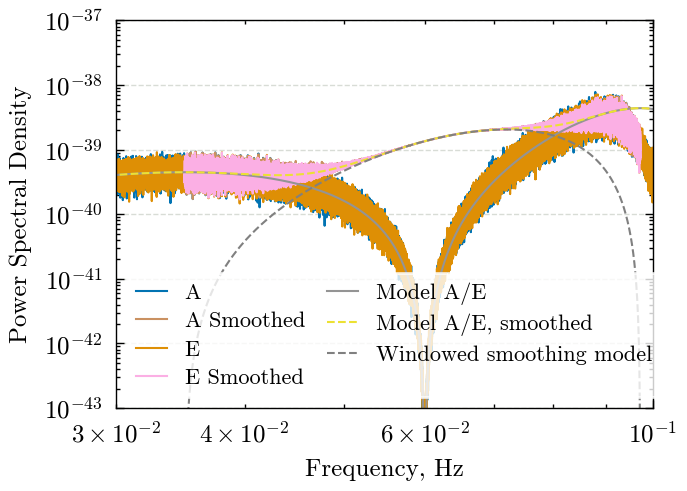
\includegraphics[width=\columnwidth]{images/dataset/figure_X_smoothing_60mHz.png}
    \caption{
        The method used to smooth over the dip in the PSD at 60 mHz.
        We draw a straight line between the two peaks either side of this point, and smoothly
        This ensures that there are no immediate jumps in the PSD to cause spectral leakage.
        transition betweem the estimated PSD and the straight line using a Hann window.
        This is applied to both the estimated and modelled PSDs used in later analysis.
    }
    \label{fig:smoothing}
\end{figure}

